\documentclass[titlepage]{article}
\usepackage{babel}
\usepackage{amsmath}
\usepackage{amssymb}
\usepackage{amsthm}
\usepackage{multicol} %spalten in seite
\usepackage{graphicx} %bilder einfügen
\usepackage[normalem]{ulem} %durchstreichen
\usepackage{tabto} %tabulator mit \tab
\usepackage{hyperref}
\usepackage{tikz}
\usetikzlibrary{automata, arrows.meta, positioning} % automaten zeichnen
\usetikzlibrary{shapes.geometric}
\usepackage{wasysym}
\usepackage{bbm}
\usepackage{bbold}
\usepackage{xcolor}
\usepackage[T1]{fontenc}
\usepackage{mathrsfs}  
\usepackage[utf8]{inputenc}
\usepackage{listings} %quellcode
\pagestyle{plain}
\pagenumbering{arabic}
\renewcommand{\arraystretch}{1.3} %vertikaler abstand von tabellen
\newcommand{\n}{\newline}
\usepackage[left=20mm, right=15mm, top=25mm, bottom=7mm, paper=a4paper]{geometry}

\renewcommand{\contentsname}{Inhaltsverzeichnis}

\renewcommand{\]}{\right]}
\renewcommand{\[}{\left[}
\renewcommand{\)}{\right)}
\renewcommand{\(}{\left(}
\renewcommand{\|}{\;|\;}

\begin{document}
	
	\begin{center}
		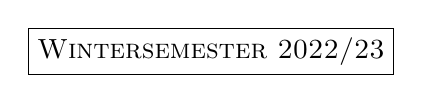
\begin{tikzpicture}
			\draw (0,0) node[draw, rectangle]{\textsc{Wintersemester 2022/23}};
		\end{tikzpicture}
		\hrulefill\\
		\begin{center}
			\LARGE\textsc{Automaten und Berechenbarkeit - Übung 02} \normalsize\\
		\end{center}
		\hrulefill
		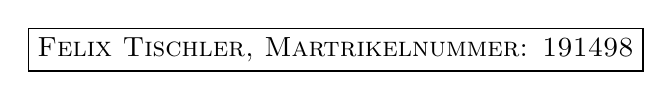
\begin{tikzpicture}
			\draw (0,0) node[draw, rectangle]{\textsc{Felix Tischler, Martrikelnummer: 191498}};
		\end{tikzpicture}
		\date{\today}
	\end{center}


	\section*{Aufgabe 1}
		\paragraph{(a)} $L_1=\{w\in\{0,1\}^*:w\text{ enthält 110 nicht als Teilwort}\}$
		\begin{align*}
			G_1=(\{0,1\},\{S,E,F\},S,R)&&&&&&&&&&&\\
			\text{mit }R:
			\begin{cases}
				S&\rightarrow S0\|E1\|\lambda\|0\|1\\
				E&\rightarrow F1\|S0\|1\|0\\
				F&\rightarrow F1\|1\|\lambda    
			\end{cases}
		\end{align*}
		\begin{proof}[Beweis] $"\subseteq"$
			Jedes Wort startet bei S.  In S können beliebig viele Nullen entstehen, oder abgebrochen werden mit $\lambda$, 0 oder 1. Wenn eine 1 erstellt wird und nicht abgebrochen wird, dann ist man in E. In E kann man mit 0,1 abbrechen oder beliebig Nullen erstellen. Sollte man in E eine Null erstellen und nicht abbrechen, dann landet man in F. In F sind keine Nullen mehr erlaubt, da jetzt das Wort die Form $(a,b)^*11$ besitzt. Somit ist 110 nicht als Teilwort erzeugbar. In F kann entweder mit $\lambda$ oder 1 abgebrochen werden. Oder man kann beliebig viele Einsen erzeugen bevor man abbricht.
		\end{proof}
		\begin{proof}[Beweis] $"\supseteq"$ "jedes Wort ist erzeugbar"
			Siehe Anhang Automat zu Aufgabe 1 (a)
		\end{proof}
		
		
		
		\paragraph{(b)} $L_2=\{w\in\{a,b\}^*:\text{der erste und der letzte Buchstabe sind in w sind gleich}\}$
			\begin{align*}
			G_2=(\{a,b\},\{S,A_1,A_2,B_1,B_2\},S,R)&&&&&&&&&&&\\
			\text{mit }R:
			\begin{cases}
				S&\rightarrow aA_1\|bB_1\\
				A_1&\rightarrow aA_1\|bB_2\|a\\
				A_2&\rightarrow b\|bB_1\|aA_2\\
				B_1&\rightarrow bB_1\|aA_2\|b\\
				B_2&\rightarrow a\|aA_1\|bB_2
			\end{cases}
		\end{align*}
		\begin{proof}[Beweis] $"\subseteq"$
			Alle Wörter starten in S. Wenn a der erste Buchstabe ist geht es in $A_1$ weiter. Andernfalls in $B_1$. Von $A_1$ kann mit a beendet werden, oder ein weiteres a erzeugt werden oder ein b hinzugefügt werden. Wenn letzteres passiert geht man in $B_2$ die 2 in $B_2$ signalisiert, dass das b nicht der orginale Buchstabe war. Somit kann nur mit beendet werden oder ein b reproduziert werden (wobei man in $B_2$ dann wieder ist) oder mit einem a zu $A_1$ wieder gelangen. Die Argumentation gilt analog wenn man mit b starten würde.
		\end{proof}
		\begin{proof}[Beweis] $"\supseteq"$
			Siehe Anhang Automat zu Aufgabe 1 (b)
		\end{proof}
		
		
		\paragraph{(c)} $L_3=\{w\in\{a,b\}^*:\text{unter den ersten drei Buchstaben in w ist mindestens ein a}\}$
			\begin{align*}
			G_3=(\{0,1\},\{S,A,B_1,B_2,E\},S,R)&&&&&&&&&&&\\
			\text{mit }R:
			\begin{cases}
				S&\rightarrow aE\|bB_1\\
				B_1&\rightarrow aE\|bB_2\\
				B_2&\rightarrow aE\\
				E&\rightarrow a\|b\|\lambda\|aE\|bE
			\end{cases}
		\end{align*}
		\begin{proof}[Beweis] $"\subseteq"$
			Alle Wörter starten bei S. Da die ersten 3 Buchstaben direkt in den ersten 3 Iterationen entstehen ist es notwendig die Bedingung mindestens ein a zu haben in diesen zu erfüllen. Somit kann man in S mit einem a beenden, oder mit einem a in $E$ gelangen oder mit einem b zu $B_1$ gelangen. In E ist die Bedingung erfüllt, da man beim ersten Übergang in E immer ein a Benötigt und innerhalb der ersten 3 Iterationen zwingend in E landet. Somit kann man in E mit einem a, b oder $\lambda$ beenden, oder beliebig a und b reproduzieren. Wenn man in $B_1$ ist, dann ist der erst Buchstabe b. Entweder beendet man mit einem a, oder man erzeugt ein a und geht dabei in E, oder man erzeugt ein weiteres b und gelangt in $B_2$. In $B_2$ muss man zwingend ein a erzeugen beim Übergang in E oder mit einem a beenden. Da die ersten 2 Buchstaben ein b sind.
		\end{proof}
		\begin{proof}[Beweis] $"\supseteq"$
			Siehe Anhang Automat zu Aufgabe 1 (c)
		\end{proof}
\end{document}